\chapter{Templates}

In order to introduce the user to a first use of the model, two examples are provided to illustrate how to start a simulation and obtain results. The key ideas embedded in the input-out structure are flexibility and self-explanatory names for variables and files.

All input-output parameters and the simulation control parameters are given in the {\it geotop.inpts} file. A log-file is generated as a track of the simulation, it summarizes the parameter set chosen for the simulation and the time evolution, i.e. the percentage of simulation completed and the amount of time required to complete it. If the simulation is long or convergency problems are encountered, this file can be very large.
If the simulation is completed a  {\it SUCCESSFUL-RUN} empty file is created, alternatively a {\it FAILED} file is printed out.
If the simulation is rerun new files are generated and old files are renamed with .old

Default values are assigned to several variables, assuming the simulation is 3D, if the users wants to change the default status, appropriate flags need to be assigned.

%=============================================================%
\section{1D simulation}
%=============================================================%
Some processes are mainly 1-dimensional, therefore they can be investigated using GEOtop in a simplified manner. In such a way the computational domain is reduced to one vertical column aligned to a Cartesian grid.
Processes related to soil temperature and snow profiles can be studied in one dimension.

Input-output and controlling simulation parameters are assigned in the \emph{geotop.inpts} file, together with the keyword specific for the 1D simulation. In order to traduce a real case study into a scheme that can be handed by the model, the following elements have to be set:
\begin{itemize}
\item [-] computational domain;
\vspace{-0.2cm}
\item [-] initial conditions;
\vspace{-0.2cm}
\item [-] boundary conditions;
\vspace{-0.2cm}
\item [-] meteorological forcing;
\vspace{-0.2cm}
\item [-] soil and snow thermic parameters.
\end{itemize}

The {\bf computational domain} is set assigning the number of layers and their thickness in the SOIL PARAMETERS block (SoilLayerThicknesses). 

The {\bf initial conditions} can be assigned to soil, snow, watertable, ice and bedrock (Table \ref{tab:IC}). Initial conditions on soil temperature are assigned through the InitSoilTemp parameter in the SOIL PARAMETERS block, the initial conditions on snow are assigned through four parameters initial snow water equivalent (InitSWE), initial snow density (InitSnowdensity), initial snow temperature (InitSnowTemp), initial snow age (InitSnowAge). The initial watertable height can be defined through the InitWaterTableHeightOverTopoSurface parameter, which takes negative value if the soil in unsaturated and 0 if it is saturated. Initial condition on ice depth, temperature and ice density can be set through the corresponding parameters InitGlacierDepth, InitGlacierDensity and InitGlacierTemp.

\begin{table}[h!]
\begin{center}
\begin{tabular}{|p{2.0cm}|p{5.5cm}|p{6.0cm}|}
\hline 
 &  \bfseries{Physical variables} & \bfseries{ Parameter name}\\
\hline 
Soil &  soil temperature & InitSoilTemp \\
& soil pressure& InitSoilPressure\\
\hline 
Snow &   snow water equivalent & InitSWE \\
& snow density & InitSnowDensity\\
& snow age & InitSnowAge\\
\hline Ice  &  ice depth & InitGlacierDepth \\
&ice density &InitGlacierDensity \\
&ice temperature & InitGlacierTemp\\
\hline Water & watertable depth & InitWaterTableHeightOverTopoSurface \\
&water pressure within the bedrock  &InitSoilPressureBedrock \\
& temperature of the bedrock & InitSoilTempBedrock \\
\hline
\end{tabular}
\caption{Synoptic table of the initial conditions}\label{tab:IC}
\end{center}
\end{table}

Dirichlet {\bf boundary conditions} are assigned at the bottom boundary of the computational domain by setting the depth at which the temperature fluctuation due to external forcing is zero (ZeroTempAmplitDepth) and providing the constant temperature at such a  depth (ZeroTempAmplitTemp). Both parameters can be found in the ENERGY BALANCE PARAMETERS block.
Boundary conditions for the mass balance (Richards equation) are set by default to no flux (as reported in the log-file).

{\bf Meteorological forcing} are assigned through the meteo-file, the horizon meteo-file and some parameters which specify the characteristic of the meteorological station and the sensor height in the METEO PARAMETERS block. There is one horizonmeteo file per meteorological station; they can be present to improve the shadow calculation.  It describes the obstacles around the station in terms of two angles; one describes the angle on an horizontal plane between the North and the object; the other angle describes the height of the object along the vertical plane.

{\bf Soil and snow thermic parameters} are assigned for each layer in the SOIL and SNOW block through several parameters such as soil thermal conductivity and capacity (ThermalConductivitySoilSolids, ThermalCapacitySoilSolids).
In addition, land cover characteristic are given in the LAND COVER PARAMETERS block.

\subsection{Parameter file: {\it geotop.inpts}}

Parameters are organized in 10 blocks; they can be flags which enable or disable functionalities in the simulation, keywords or values. The 10 blocks are listed in the followings:
 
 \begin{enumerate}
\item Base Parameters (Table \ref{tab:baseParameters}). This block contains 4 parameters which define the integration interval, the simulated time through the initial and end dates and whether the simulation has to be run more than one time; 3 flags defining whether the water and/or the energy balance calculations have to be switch on (1) and whether the simulation is 1D. The default case is 3D simulation which corresponds to setting the {\it PointSim} to 0 or, alternatively, not using it. The last two parameters are defined by the users.

\item  Input files and Headers (Table \ref{tab:inputHeader}). This block contains the keywords which define the column names for some input files, such as the meteo file, the horizon meteo file and the list point file.

\item  Meteo Parameters: define the characteristics of the meteorological station/s. (Figure \ref{meteoPAR})
\item  Energy Balance Parameters (Table \ref{tab:energyBalance}). These parameters are necessary to solve the energy balance equation.
\item Water Balance Parameters (Table \ref{tab:energyBalance}). These parameters are necessary to solve the Richards equation.
\item Land Cover Parameters (Table \ref{tab:landCoverPar}). These parameters allow for the surface roughness, reflectivity and emissivity characterization.

\item  Soil Parameters (Table \ref{tab:soilPar}). These parameters allow the user to characterize the soil both in terms of geometry (number of layers and thickness) and hydraulic properties (van Genucten [1980] parameters).

\item Snow Parameters (Table \ref{tab:snowPar}). These parameters allow for snow characterization.

\item Output in a Point and Output Time Series (Figure \ref{output}) allow the user to define which output has to be printed and in which format.
\end{enumerate}


 For additional details see Tables ... \textcolor{red}{Add REF to keyword table}.
%========== Base Parameters ==============
\begin{table}[h!]
\begin{center}
\begin{tabular}[c]{|c|c|}
\hline
Parameter / Keyword / Flag & value\\
\hline
TimeStepEnergyAndWater& 3600\\
InitDateDDMMYYYYhhmm  & 12/07/2010 00:00 \\
EndDateDDMMYYYYhhmm & 15/08/2010 23:00\\
NumSimulationTimes  & 1\\
WaterBalance & 1\\
EnergyBalance& 1\\
PointSim & 1\\
StandardTimeSimulation & 0 \\
DtPlotPoint & 1 \\
\hline
\end{tabular}
\caption{Base Parameters.}
\label{tab:baseParameters}
\end{center}
\end{table}
%=========== File names and Header parameters ===========
\begin{table}[h!]
\begin{center}
\begin{tabular}[c]{|c|c|}
\hline
Parameter / Keyword / Flag & value\\
\hline
PointFile& "listpoints" \\
HeaderPointElevation  & "ele" \\
HeaderPointSlope & "slp"\\
HeaderPointAspect  & "asp"\\
HeaderPointSkyViewFactor & "sky"\\
HeaderPointMaxSWE & "swe"\\
\hline
MeteoFile & "meteo"\\
HeaderDateDDMMYYYYhhmmMeteo & "date" \\
HeaderWindVelocity & "WindS" \\
HeaderWindDirection & "WindDir" \\
HeaderWindX & "WindX"\\
HeaderWindY &"WindY"  \\
HeaderRH & "RelHum"\\
HeaderAirTemp & "AirT" \\
HeaderSWglobal & "SWglobal"\\
HeaderIPrec & "Iprec" \\
HeaderCloudSWTransmissivity & "CloudTrans" \\
\hline
HorizonMeteoStationFile & "horizonmeteo"\\
HeaderHorizonAngle & "Angle" \\
HeaderHorizonHeight & "Height"\\
\hline
\end{tabular}
\caption{Input files and headers}
\label{tab:inputHeader}
\end{center}
\end{table}
%=========== Energy Balance Parameters
\begin{table}[h!]
\begin{center}
\begin{tabular}[c]{|c|c||c|c|}
\hline
\multicolumn{2}{|c||}{Energy balance} & \multicolumn{2}{|c|}{Water balance}\\
\hline
Parameter / Keyword / Flag & value& Parameter / Keyword / Flag & value\\
\hline
LWinParameterization & 9 & FrozenSoilHydrCondReduction & 2\\
MoninObukhov & 1&  RichardTol & 1.E-8 \\
HeatEqTol & 1.E-5 & RichardMaxIter & 500\\
HeatEqMaxIter & 500 & RichardInitForc & 0.01 \\
ZeroTempAmplitDepth & 20100 &&\\
ZeroTempAmplitTemp & -1.25 &&\\
\hline
\end{tabular}
\caption{Parameters  used for solving the energy balance and Richards equation.}
\label{tab:energyBalance}
\end{center}
\end{table}

\vspace{-1.0cm}
%=========== Water Balance Parameters
%\begin{table}[h!]
%\begin{center}
%\begin{tabular}[c]{|c|c|}
%\hline
%Parameter / Keyword / Flag & value\\
%\hline
%FrozenSoilHydrCondReduction & 2 \\
%RichardTol & 1.E-8 \\
%RichardMaxIter & 500 \\
%RichardInitForc & 0.01 \\
%\hline
%\end{tabular}
%\caption{Parameters  used for solving Richards equation.}
%\label{tab:waterBalance}
%\end{center}
%\end{table}

\vspace{-1.0cm}
%=======Landcover Parameter
\begin{table}[h!]
\begin{center}
\begin{tabular}[c]{|c|c|}
\hline
Parameter / Keyword / Flag & value\\
\hline
SoilRoughness & 100 \\
ThresSnowSoilRough & 5 \\
AlbExtParSnow & 3 \\
SoilAlbVisDry & 0.5 \\
SoilAlbNIRDry & 0.5 \\
SoilAlbVisWet & 0.5 \\
SoilAlbNIRWet & 0.5 \\
SoilEmissiv & 0.96 \\
\hline
\end{tabular}
\caption{Land cover characterization parameters}
\label{tab:landCoverPar}
\end{center}
\end{table}

\vspace{-1.5cm}
%=======Soil Parameters
\begin{table}[h!]
\begin{center}
\begin{tabular}[c]{|c|c|}
\hline
Parameter / Keyword / Flag & value\\
\hline
SoilLayerTypes & 1 \\
InitWaterTableHeightOverTopoSurface & -3000 \\
SoilLayerThicknesses &100,100,100, ... \\
InitSoilTemp & 0.34, 0.15, -0.03, ... \\
VerticalHydrConductivity & 0.0001 \\
ThetaRes & 0 \\
ThetaSat & 0.2,0.2,0.2,0. .... \\
AlphaVanGenuchten & 0.0436,0.0436,0.0436, .... \\
NVanGenuchten & 1.51,1.51,1.51, ... \\
ThermalConductivitySoilSolids & 2.3 \\
ThermalCapacitySoilSolids & 2.3E+06 ... \\
\hline
\end{tabular}
\caption{Soil   characterization parameters}
\label{tab:soilPar}
\end{center}
\end{table}
%=======Snow Parameters
\begin{table}[h!]
\begin{center}
\begin{tabular}[c]{|c|c|}
\hline
Parameter / Keyword / Flag & value\\
\hline
FreshSnowReflVis&0.96 \\
FreshSnowReflNIR&0.72 \\
BlowingSnow&0 \\
InitSWE & 0 \\
InitSnowDensity & 180 \\
InitSnowTemp & -3 \\
InitSnowAge & 0 \\
\hline
NumMaxSnowLayers & 5 \\
InfiniteSnowLayer & 3 \\
MinLayerThicknessSnow & 5,  30,  120,  5,  5 \\
MaxLayerThicknessSnow & 20, 100, 10000, 100, 50 \\
\hline
RainCorrFactor &1 \\
SnowCorrFactor &1.6 \\
\hline
SnowSMIN &25 \\
SnowSMAX &70 \\
SnowCURV &-150 \\
\hline
DewTempOrNormTemp & 0.65 \\
ThresTempRain & 2 \\
ThresTempSnow & -1 \\
SnowEmissiv & 0.94 \\
\hline
SnowRoughness & 0.1 \\
FreshSnowReflVis & 0.9 \\
FreshSnowReflNIR & 0.65 \\
IrriducibleWatSatSnow & 0.02 \\
MaxSnowPorosity &0.7 \\
DrySnowDefRate & 1 \\
SnowDensityCutoff & 100 \\
WetSnowDefRate & 1.5 \\
SnowViscosity & 1.E6 \\
AlphaSnow & 1.E2 \\
\hline
\end{tabular}
\caption{Snow characterization parameters}
\label{tab:snowPar}
\end{center}
\end{table}
\clearpage

%=================INPUT FILES ===============
\subsection{Input files}
The input files required to run a 1D-simulation in addition to the {\it geotop.inpts} file are the followings:
\begin{itemize}
\item [-] meteo file;
\item [-] horizon meteo file;
\item [-] list point.
\end{itemize}
The {\bf meteo file} contains a time series of  meteorological data. If data for more stations are available, one meteo file per station needs to prepared before a simulation can be run; the same holds for the horizionfile. Using the meteo parameters in  the {\it geotop.inpts} file the user can specify the number of stations and their characteristics, e.g. location, elevation, sky view factor, time shift with respect to UTC if any and sensors height. In case of more stations, scalar values are substituted by vectors (Figure \ref{meteoPAR}). For flexibility purposes the user can specify the columns name of the meteo file through the keywords provided in the Input files and Header block in the {\it geotop.inpts} file, as shown in Figure \ref{inputHeader}. The quoted names to the right can be changed at the user's convenience. The same concept applies to the horizon meteo and list point files, whose column names can be defined through appropriate keywords (Figure \ref{inputHeader}).

The {\bf horizon file} it describes the obstacles around the station in terms of two angles; one describes the angle on an horizontal plane between the North and the object; the other angle describes the height of the object along the vertical plane.

The {\bf list point} file describes the morphological features of the points where the simulation is performed. If more than one point are listed in this file the simulation is run simultaneously run at multiple points.  The features that have to be provided for each point are the point identification number, the elevation, the local slope, the aspect and the sky view factor.

\begin{figure}[h!]
\begin{center}
{\includegraphics[width=.48\columnwidth]{./images/pic_template/meteoPARAM_1stazione.png}} \quad
{\includegraphics[width=.48\columnwidth]{./images/pic_template/meteoPARAM_stazioni.png}} \\
\caption{Example of meteo parameter sets, for one station on the left, for 3 station on right.}
\label{meteoPAR}
\end{center}
\end{figure}

\begin{figure}[!h]
\begin{center}
   \includegraphics[width=0.7\textwidth]{./images/pic_template/InputFile&Headers.png}
    \caption{Input file Headers block in the {\it geotop.inpts} file} \label{inputHeader}
\end{center}
\end{figure}
%=================OUTPUT FILES ===============
\subsection{Output files}
The number and the type of output that GEOtop prints out can be decided by the user through the DefaultPoint parameter. If this is set  to 1, GEOtop prints out all possible output, as listed in Table ... \textcolor{red}{Add REF to keyword table}; alternatively, the user can specify which output wants GEOtop to print by setting the DefaultPoint parameter to 0. In this case the headers of the wanted output have to be specified as well (Figure \ref{output}). This section of the parameter file allows the user to change the column name and position in the output files by using the appropriate keyword. e.g. IDPointPoint will be printed on column 4 and labeled {\it chose a name}. In the example shown in Figure \ref{output}, 22 columns will be printed into the file named point, as specified by the PointOutputFileWriteEnd keyword. This name can be defined by the user.
In the presented example two are the output files {\it point.txt} and {\it soiTave.txt}. This is an option that can be decided by the users and additional files can be printed on demand.

\begin{figure}[!h]
\begin{center}
   \includegraphics[width=0.7\textwidth]{./images/pic_template/output_PAR.png}
    \caption{Output blocks in the {\it geotop.inpts} file defining column header and their position in the output file} \label{output}
\end{center}
\end{figure}

\clearpage
%=============================================================%
\section{3D distributed simulation}
%=============================================================%
GEOtop can reproduce physical processes which are mainly characterized by 3D-dynamics, such as snow melt in  mountainous area, atmosphere-vegetation interactions and soil-atmosphere interaction (in bare soil), infiltration, water redistribution through the soil and stream discharge generation (Figure \ref{processi3D}). Such processes required the topography of the study area to be given as input to the model and mass balance equation to solved in three dimensions (energy balance equation is solved 1D given the prevailing vertical fluxes to horizontal). GEOtop uses a 3D-structured grid as shown in Figure \ref{3Dscheme}.
In addition, to investigate interactions between atmosphere and vegetation, and between soil and atmosphere, distributed information on landcover and soil type are required. 

%==3D pictures
\begin{figure}[h!]
\begin{center}
{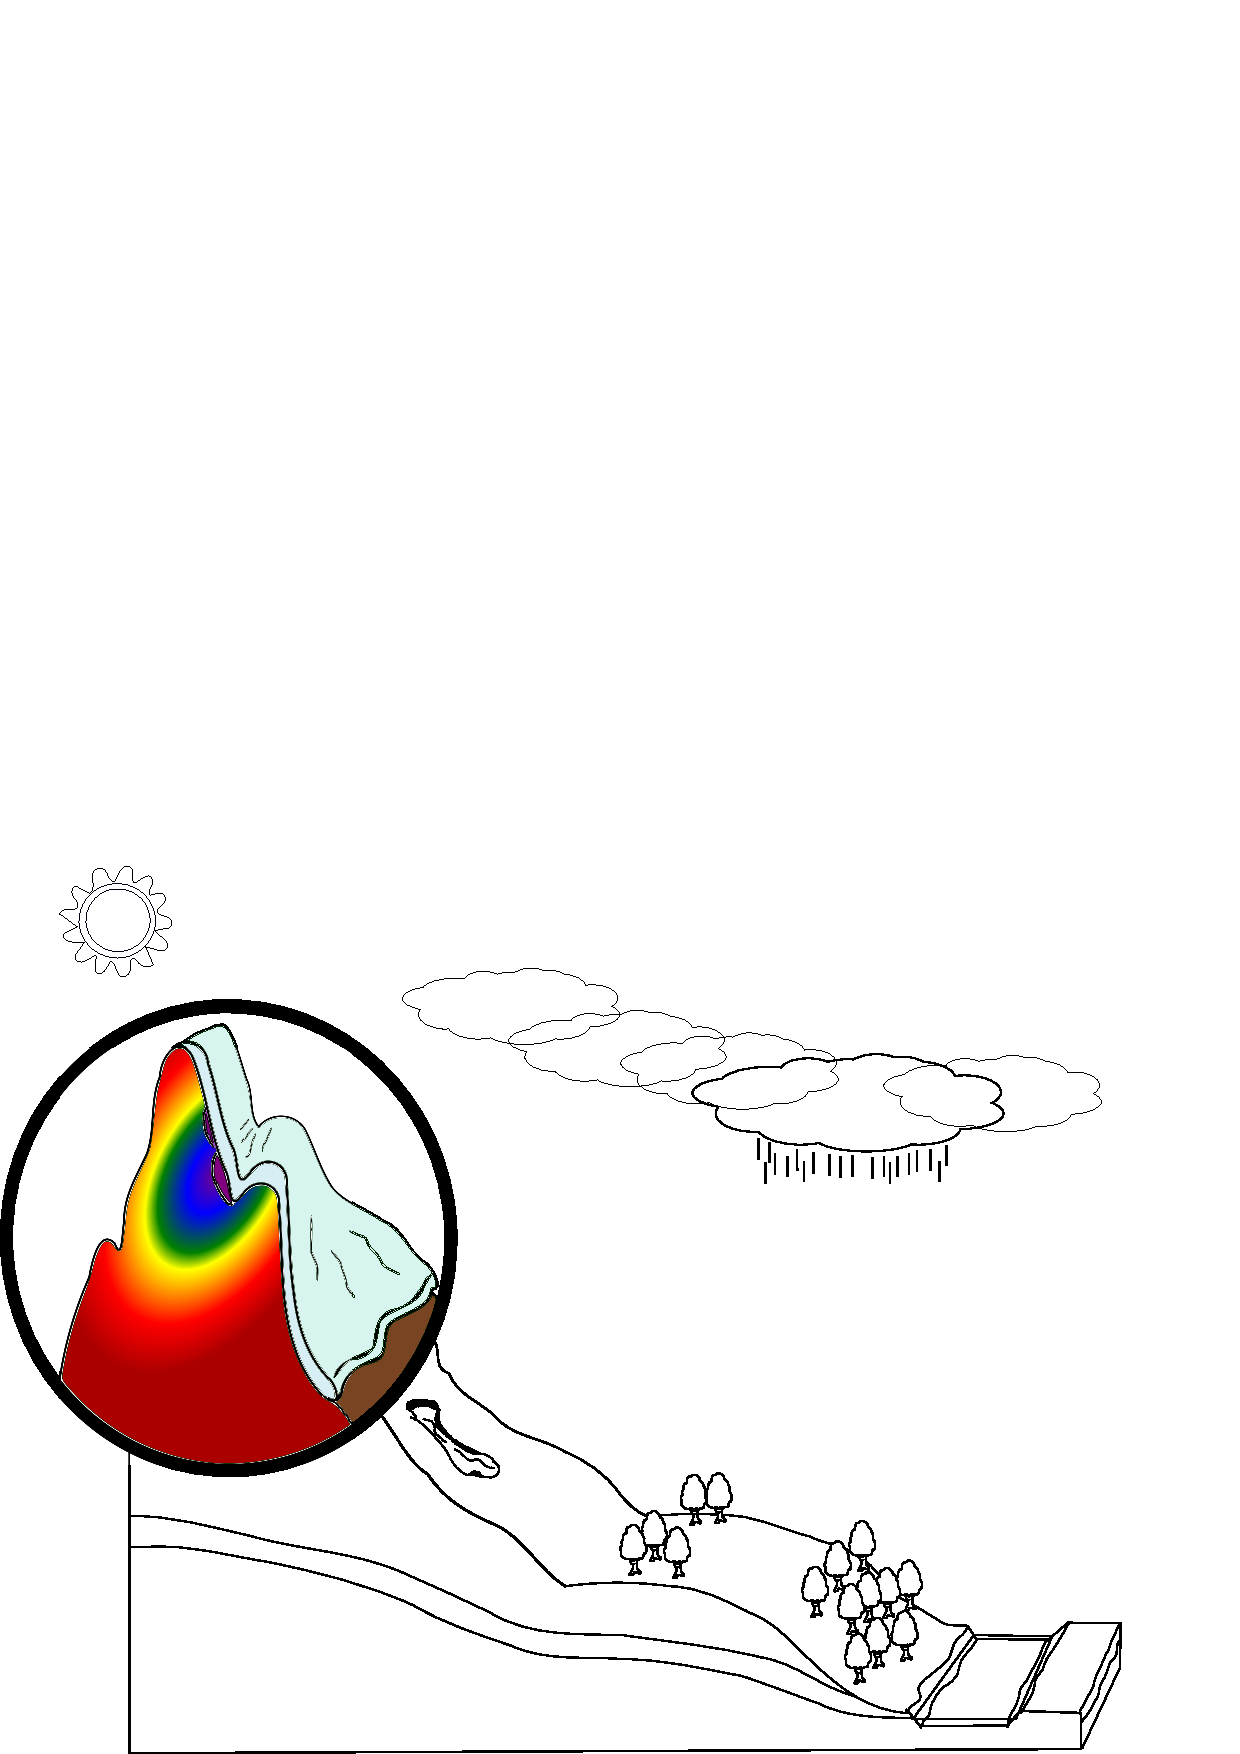
\includegraphics[width=.48\columnwidth]{./images/pic_template/criosfera_temp_grad.png}} \quad
{\includegraphics[width=.48\columnwidth]{./images/pic_template/vegetazione.pdf}} \\
{\includegraphics[width=.48\columnwidth]{./images/pic_template/suolo.pdf}} \quad
\caption{Physical processes typical of mountain hydrology which can be reproduced using a distributed, 3D model, such as GEOtop.}
\label{processi3D}
\end{center}
\end{figure}

The example presented refers to a 2 day-run on a 0.7 km$^2$ alpine watershed. Data from only one station were available for this catchment. Soil type and landcover data were derived from satellite images and soil characterization (geomechanical properties and lithologic profiles) were derived from extensive field campaigns. In this respect GEOtop is a tool to handle post-processed Earth Observation (EO) data and distributed field data.
The goal of this template is to show how the user can set up a distributed simulation.

%==3D scheme
\begin{figure}[!h]
\begin{center}
   \includegraphics[width=0.9\textwidth]{./images/pic_template/3Dscheme.pdf}
    \caption{3-dimensional grid structure implemented in GEOtop to solve the mass balance equation.} \label{3Dscheme}
\end{center}
\end{figure}

%=========PARAMETER FILE
\subsection{Parameter file}
The structure of the parameter files is analogous to what previously illustrated for the 1D case with few additional keywords and parameters which need to be add in order to print out distribute and aggregated results, such as maps and stream flow, see Table \ref{tab:baseParameters3D}. The { \it DtPloDischarge} parameter specifies the print out stream discharge time series time step in hours (1), the { \it OutputSoilMaps} parameter specifies the print out  time step for the stream discharge time series (24 hours). The barycentric latitude and longitude for the watershed has to supplied.
%========== Base Parameters 3D==============
\begin{table}[h!]
\begin{center}
\begin{tabular}[c]{|c|c|}
\hline
Parameter / Keyword / Flag & value\\
\hline
TimeStepEnergyAndWater& 3600\\
InitDateDDMMYYYYhhmm  & 12/07/2010 00:00 \\
EndDateDDMMYYYYhhmm & 15/08/2010 23:00\\
NumSimulationTimes  & 1\\
WaterBalance & 1\\
EnergyBalance& 1\\
\hline
Latitude (avg) & 46.3 \\
Longitude (avg)& 11.7 \\

StandardTimeSimulation & 0 \\
\hline
DtPloDischarge & 1 \\
DtPlotPoint & 1 \\
DtPlotBasin & 1 \\
\hline
OutputSoilMaps & 24 \\
OutputSnowMaps & 24 \\
OutputSurfEBALMaps & 24 \\
OutputMeteoMaps & 24 \\
\hline
\end{tabular}
\caption{Base Parameters for a 3D simulation. Units are specified in Table \textcolor{red}{ADD REF TO KEYWORD TABLE}}
\label{tab:baseParameters3D}
\end{center}
\end{table}

%=========== File names and Header parameters ===========
Raster file maps name have to be specified in the File names and Header parameters section as shown in Table \ref{tab:inputHeader3D}. The number of available meteorological stations and their characteristics have to be specified in the appropriate parameter section. 

\begin{table}[h!]
\begin{center}
\begin{tabular}[c]{|c|c|}
\hline
Parameter / Keyword / Flag & value\\
\hline
PointFile& "listpoints" \\
HeaderPointElevation  & "ele" \\
HeaderPointSlope & "slp"\\
HeaderPointAspect  & "asp"\\
HeaderPointSkyViewFactor & "sky"\\
HeaderPointMaxSWE & "swe"\\
\hline
MeteoFile & "meteo"\\
HeaderDateDDMMYYYYhhmmMeteo & "date" \\
HeaderWindVelocity & "WindS" \\
HeaderWindDirection & "WindDir" \\
HeaderWindX & "WindX"\\
HeaderWindY &"WindY"  \\
HeaderRH & "RelHum"\\
HeaderAirTemp & "AirT" \\
HeaderSWglobal & "SWglobal"\\
HeaderIPrec & "Iprec" \\
HeaderCloudSWTransmissivity & "CloudTrans" \\
\hline
DEMfile & "dem"\\
LandCoverMapFile & "landcovermapfile" \\
SkyViewFactorMapFile & "0sky"\\
SlopeMapFile & "0slope" \\
AspectMapFile & "0aspect" \\
CurvaturesMapFile & "0curvature" \\
SoilMapFile & "soiltype" \\
SoilParFile & "soil/soil" \\
\hline
\end{tabular}
\caption{Input files and headers for a spatially distributed simulation.}
\label{tab:inputHeader3D}
\end{center}
\end{table}

%=======Soil Parameters
The number of landcover and soil type categories have to be specified in the appropriate parameter section. 
In case the soil in the watershed is not homogeneous, the number of different soil type can be assigned to the SoilLayerTypes parameter (see Table \ref{tab:soilPar3D}) and a description for each soil type has to be provided. This is done through files stored in a user defined path specified by the keyword {\it SoilParFile} (Table \ref{tab:inputHeader3D}). Soil characterization files must contain information on the layer thickness, hydraulic conductivity, residual and saturated moisture content etc. as specified by the keywords in Table \ref{tab:soilPar3D}. 

In addition to what already said for the 1D case, distributed {\bf Initial conditions} (IC) can be assigned using raster maps associated with a specific keyword which specifies the path to the file. E.g. the IC on the water table depth can be assigned through the keyword {\it InitWaterTableHeightOverTopoSurfaceMapFile}, the IC on initial snow height and initial ice depth  can be assigned through the keywords {\it InitSnowDepthMapFile} and {\it
InitGlacierDepthMapFile}. 

In addition to what already said for the 1D case, lateral {\bf boundary conditions} can be assigned through the keyword { \it FreeDrainageAtLateralBorder}.
%========Soil Parameters TABLE
\begin{table}[h!]
\begin{center}
\begin{tabular}[c]{|c|c|}
\hline
Parameter / Keyword / Flag & value\\
\hline
SoilLayerTypes & 28 \\
InitWaterTableHeightOverTopoSurface & -1000 \\
InitSoilTemp & 5 \\
ThermalConductivitySoilSolids & 2.5 \\
ThermalCapacitySoilSolids & 2.3E6 \\
\hline
HeaderSoilDz & "Dz" \\
HeaderLateralHydrConductivity & "Kh" \\
HeaderNormalHydrConductivity & "Kv" \\
HeaderThetaRes & "res" \\
HeaderFieldCapacity & "fc" \\
HeaderThetaSat & "sat" \\
HeaderAlpha & "a" \\
HeaderN & "n" \\
HeaderSpecificStorativity & "SS" \\
\hline
\end{tabular}
\caption{Soil characterization parameters for a 3D simulation}
\label{tab:soilPar3D}
\end{center}
\end{table}

\vspace{-1.5cm}

%==3D output keyword
\begin{figure}[h!]
\begin{center}
   \includegraphics[width=0.55\textwidth]{./images/pic_template/output_PAR3D.png}
    \caption{Keyword setting for output files.} \label{tab:outputPAR3D}
\end{center}
\end{figure}

\clearpage
%=========INPUT
The raster maps and input files which are strictly required to run a distributed simulation are the following:

\subsection{Input maps and files}
\begin{itemize}
\item [-] Digital Elevation Model DEM.
\item [-] Landcover map
\item [-] Soiltype map and a file characterizing each different soil type (Figure \ref{soilT}).
\item [-] Time series of meteorological forcing.
\end{itemize}
To improve the quality of the simulation additional raster maps derived from geomorphological analysis of the DEM can be supplied. These maps detail the morphology of the watershed allowing for more reliable calculations. These maps are: slope and aspect maps, curvatures along specified directions and a drainage direction map. They can by computed through sounded hydrological routines such as the Horton Machines \textcolor {red} {ADD REFERENCES}.
%==DEM
\begin{figure}[h!]
\begin{center}
   \includegraphics[width=0.8\textwidth]{./images/pic_template/dem_duron.png}
    \caption{Digital elevation map of the investigated watershed.} \label{dem}
\end{center}
\end{figure}

%==TABS MEAN AIR TEMP
\begin{figure}[h!]
\begin{center}
   \includegraphics[width=0.8\textwidth]{./images/pic_template/soilType1.png}
    \caption{Example of a soil type characterization file} \label{soilT}
\end{center}
\end{figure}

The map resolution play an important role on the computational time therefore a trade-off between precision and the computational time has to be defined by the users. As a figure, the DEM used in this example is 5m resolution and counts 55648 cells in total.

%=========OUTPUT
\subsection{Outputs}
GEOtop can yield two types of different outputs:
\begin{itemize}
\item [-] raster maps
\item [-] time series (discharge, air temperature, evaporation, latent heat fluxes, etc.....) at specific points (Figure  \ref{tabs_airT}).
\end{itemize}
The output raster maps (Figure \ref{airT}) have to be specified by the user through appropriate keywords in the parameter file (see Table \ref{tab:inputHeader3D}), in addition, their output frequency has to be assigned through the {\it OutputXXXMaps} parameter.
%==MAP MEAN AIR TEMP

\begin{figure}[h!]
\begin{center}
   \includegraphics[width=0.8\textwidth]{./images/pic_template/output_airT.png}
    \caption{One of the many distributed output, the mean air temperature} \label{airT}
\end{center}
\end{figure}
%==TABS MEAN AIR TEMP
\begin{figure}[h!]
\begin{center}
   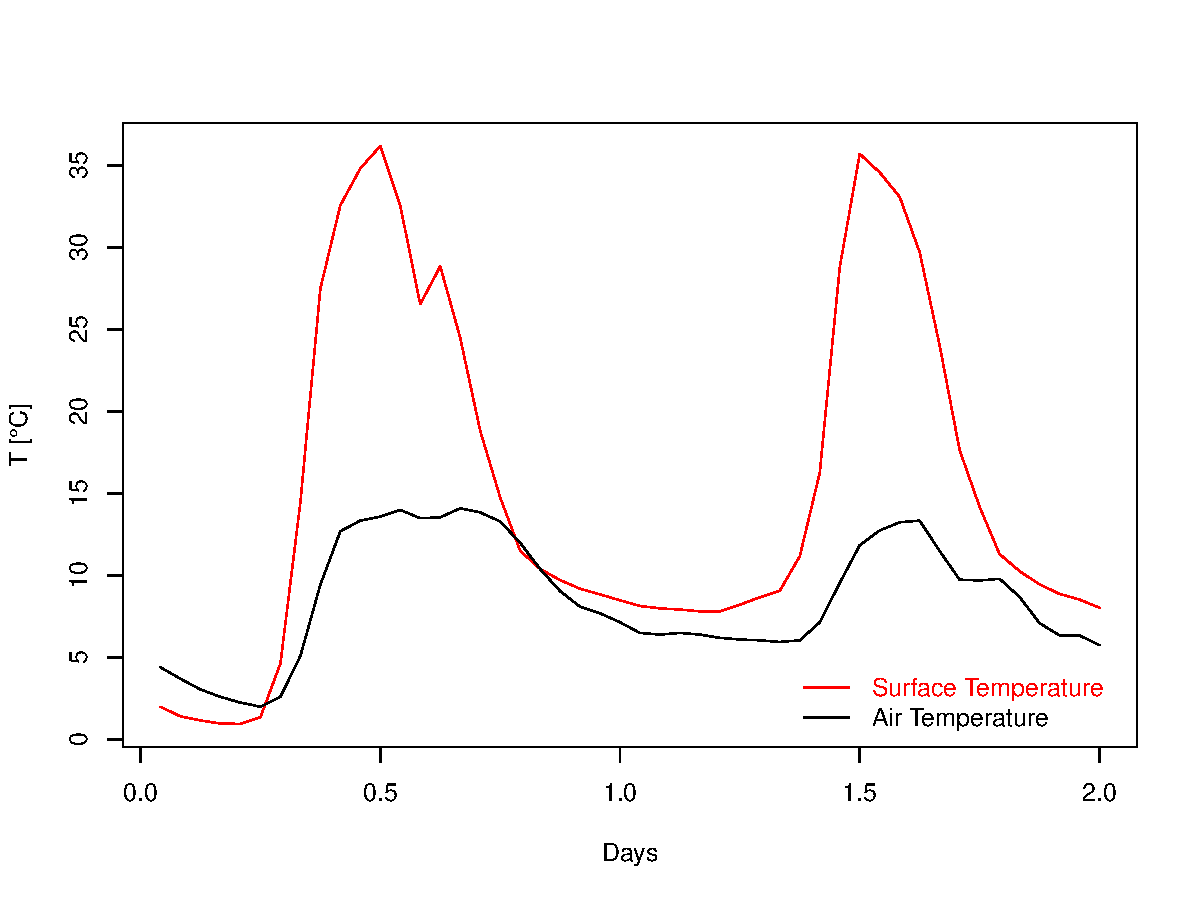
\includegraphics[width=0.8\textwidth]{./images/pic_template/tabs_airT.pdf}
    \caption{Two day-time series of mean air temperature output for a specified point} \label{tabs_airT}
\end{center}
\end{figure}






